\documentclass[12pt]{article}
\usepackage{graphicx}
\graphicspath{ {./NotesImages} }

\title{Monitoring Error-related potentials Experiment Notes}
\author{Annabelle Chan}
\date{November 2024}

\begin{document}
\maketitle
Link: https://bnci-horizon-2020.eu/database/data-sets\newline
\section{Experiment Summary}
6 participants are tasked to identifying whether a cursor on a screen are moving towards the right section on the screen (that will be signified by a colored square). During the experiment, an EEG scan will be ran as the participant accesses the situation.

Each trial lasts approximately 2000 ms and participants have no control over the cursor. Since this experiment is used to monitor erroneous actions, there is about a 0.20 probability for the cursor to move in the wrong direction.

Protocol events (cursor direction and target location) are stored in the EEG recoring. 
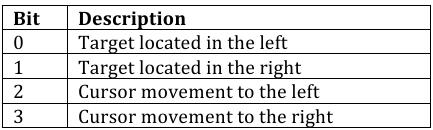
\includegraphics[scale=1]{ProtocolEventTable}
In consequence events '5' and '10' mark correct movements, while '6' and '9' mark erroneous movements.

\section{Notes on Data}
The data is in MATLAB variable format. There is experiment data from 6 participants. Each participant had two sessions with each session having 10 runs. Each run has corresponding raw eeg data (data\{i,j\}.eeg) (m samples x n channels) and recording metadata (data\{i,j\}.header). 

The metadata includes the subject number (header.Subject), the session number (header.sample), the recording sampling rate (header.SampleRate), the electrode labels (header.Label), and the recording events (header.EVENT).

\section{Notes on my experiment}
I will be using the recording events and the raw EEG data. Each sample in each run will be counted as a data point. I will use the recording events to create output data (+1 for correct direction and -1 for incorrect direction), and I will use the raw eeg data as input data. I plan to make two features for the input data.

For the raw EEG data, I will focus on the electrodes for the occipital lobe (which is used for image processing) and the frontal lobe (which is used for decision making).\newline
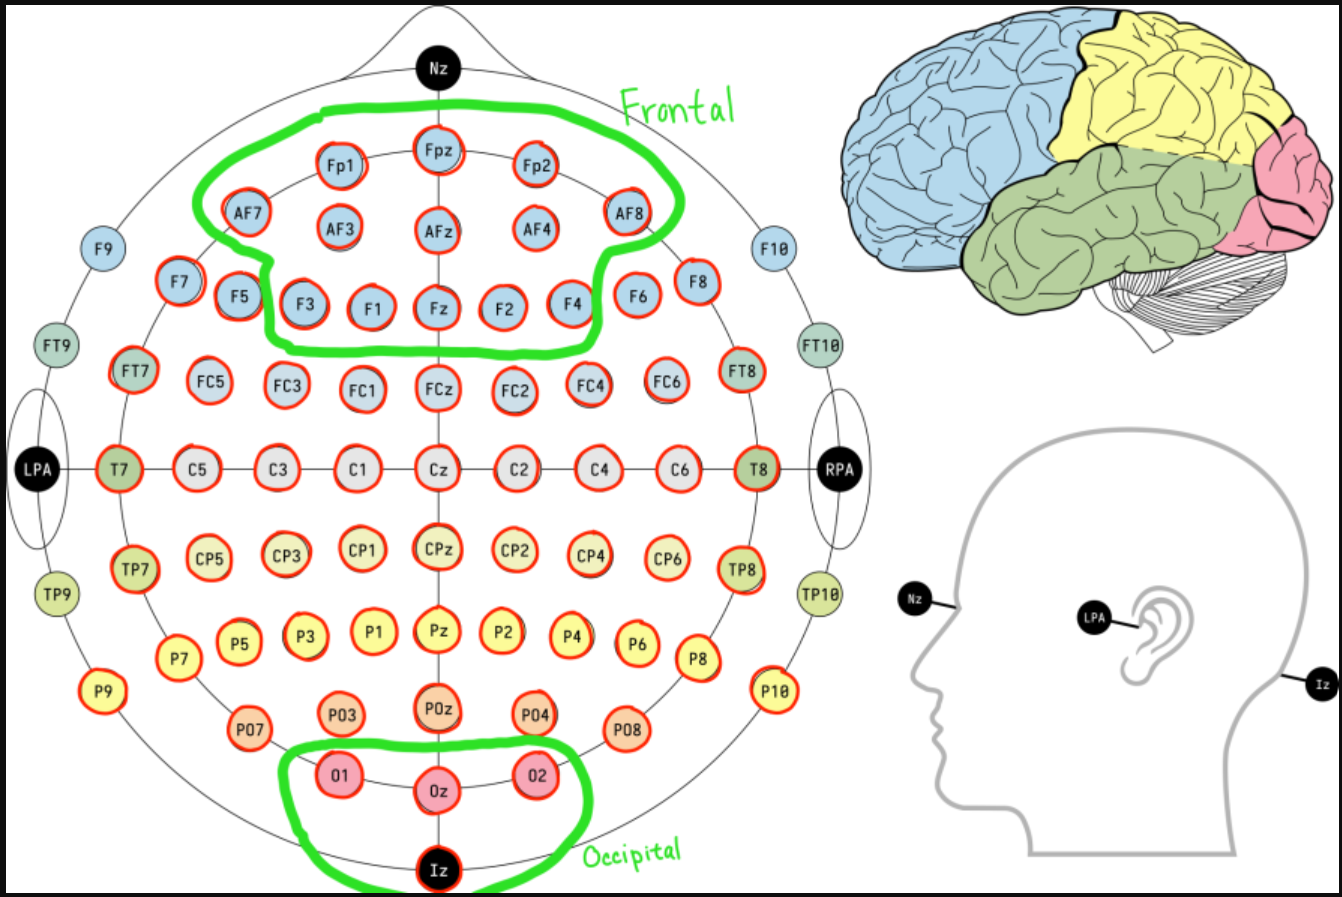
\includegraphics[scale=0.4]{ElectrodePlacements}\newline
In the above image, I've circled all the eletrodes used in the Monitoring Error-related potentials experiment in red, and circled grouped the elctrodes used in my experiment in a green circle. All the electrodes names are listed in the same order as the channels in the raw EEG data in header.label for each run. 

For the recording events, I will use Positions to locate which sample in the raw EEG data got recorded with a type. If the type is labeled with a 5 or 10, then that sample is of correct movements. If the type is labeled with a 6 or 9, then that sample is of erroneous movements. All other types will be ignored.

Reference "Organize.m"

\section{EEGLAB}
EEGLAB Download SIte: https://sccn.ucsd.edu/eeglab/downloadtoolbox.php

To start up EEGLAB, open MATLAB and change the MATLAB path to the eeglab2024.2. Next type "eeglab" in the command window and press enter. You should see the main menu.\newline
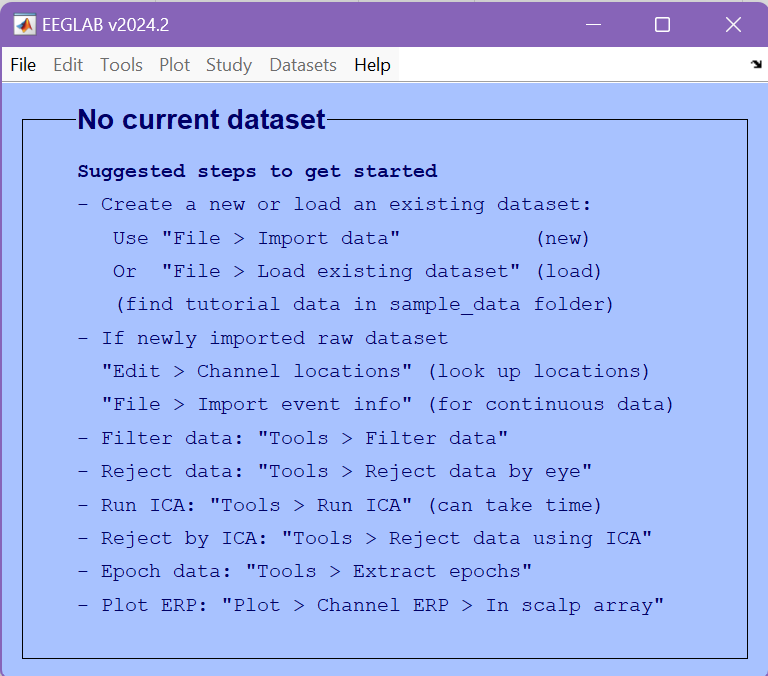
\includegraphics[scale=0.4]{EEGLABMainMenu}\newline
To restart EEGLAB, close out of the main menu. This will remove all loaded EEG datasets.

To load all the EEG data, run "LoadDataset.m" then run "loadEEGScript.m". If there are issues loading the eeglab from script, try manually loading eeglab, close out of the main menu, and then run the script. After the script finish running, there should be 120 data sets.
"LoadDataset.m" reorganizes the raw EEG data into a format that eeglab can read. Then it will create a matrix holding the event information (the first column contains the time stamp and the second column contains the event type, protocol events).
"loadEEGScript.m" will load all the datasets into the eeglab with the format "Subjectij\_rk" with i being the subject number, j being the session number, and k being the run number.

\end{document}